
\documentclass[12pt]{article}

%% Use the option review to obtain double line spacing
%% \documentclass[authoryear,preprint,review,12pt]{elsarticle}

%% Use the options 1p,twocolumn; 3p; 3p,twocolumn; 5p; or 5p,twocolumn
%% for a journal layout:
%% \documentclass[final,1p,times]{elsarticle}
%% \documentclass[final,1p,times,twocolumn]{elsarticle}
%% \documentclass[final,3p,times]{elsarticle}
%% \documentclass[final,3p,times,twocolumn]{elsarticle}
%% \documentclass[final,5p,times]{elsarticle}
%% \documentclass[final,5p,times,twocolumn]{elsarticle}

%% For including figures, graphicx.sty has been loaded in
%% elsarticle.cls. If you prefer to use the old commands
%% please give \usepackage{epsfig}

%% The amssymb package provides various useful mathematical symbols
\usepackage{amssymb}
%% The amsthm package provides extended theorem environments
%% \usepackage{amsthm}


\usepackage[dvipsnames]{xcolor}

\usepackage[margin=1in]{geometry}
\usepackage{amsmath}
\usepackage{listings}
\usepackage[T1]{fontenc}
\usepackage{geometry}

\usepackage{caption}
\usepackage{subcaption}

\usepackage[cp1252]{inputenc}
\usepackage{graphicx}
\usepackage{color}
\usepackage[normalem]{ulem}
\usepackage{soul}
\usepackage{hyperref}


\usepackage{lmodern}
\usepackage{booktabs}
\usepackage{multirow}
\usepackage[flushleft]{threeparttable}
\usepackage{multirow}

\newcommand{\modulename}[1]{\textit{#1}}
\newcommand{\note}[1]{{\color{red} #1}}
\newcommand{\code}[1]{\lstinline{#1}}
\def\arraystretch{1.5}


\lstset{language=C++,
	tabsize=2,
	basicstyle=\linespread{1}\small\ttfamily,
	backgroundcolor=\color{gray!20},
	commentstyle=\color{green!70!black},}

\newcommand{\psiv}{\vec{v}}
\newcommand{\psivdt}{\frac{\partial \psiv}{\partial t}}
\newcommand{\rhodt}{\frac{\partial \rho}{\partial t}}
\newcommand{\tdeg}{\textdegree}

\begin{document}

\title{9446B Final Project: Simulation of 864 Argons}

%% use optional labels to link authors explicitly to addresses:
%% \author[label1,label2]{}
%% \affiliation[label1]{organization={},
%%             addressline={},
%%             city={},
%%             postcode={},
%%             state={},
%%             country={}}
%%
%% \affiliation[label2]{organization={},
%%             addressline={},
%%             city={},
%%             postcode={},
%%             state={},
%%             country={}}

\author{Steven A. Silber\and 250714687}


\maketitle

%% \linenumbers

%% main text
\section{Introduction}
\label{}

Particle dynamics simulations are a key tool to understanding complex phenomena using known (or assumed!) fundamental principles of nature. Since the advent of analogue computers, programs were written to simulate the dynamics of many body systems. The particular one of interest is the simulation of liquid Argon by Rahman in 1964 to explore whether two-body dynamical interactions can explain observed spectra of scattered slow neutrons~\cite{Rahman1964}. Liquid Argon is a monoatomic species, so is a perfect candidate for simulating based on two-body dynamics. In general, there is significant scientific interest in slow neutron scattering experiments in liquids~\cite{Rahman1962}, so exploring the theoretical underpinnings of physical observations is hoped to add to this topic.
%These simulations can also be compared to experiment since liquid Argon has been the system of choice for a number of slow neutron scattering experiments~\cite{Eisenstein1942, Well1985}
% in the drive to validate models of two-body dynamical correlations scatters slow neutrons

Slow, or inelastic, neutron scattering can be used to determine the arrangement of a particular condensed matter system and study the motion of its particles. Specifically, the resulting spectrum of slow neutron scattering provides a quantity called the ``dynamic structure factor''~\cite{Squires1996Book}. Other neutron scattering techniques can reveal the structure and composition of systems, such as crystals~\cite{Feigin2013}, but we are specifically curious about slow neutron scattering. In general, dynamic structure factor is something that can be measured from simulation data and used to predict slow neutron scattering, thereby facilitating comparison with experiments~\cite{Nijboer1966}. 

However, in this work, we will not be measuring the dynamic structure factor directly, instead we will follow most of the process laid out by Rahman and compute different quantities.
%
The idea is to validate the theory of two-body dynamics by ensuring that these quantities match Rahman and experiment.
%, the objective is to test how well  
To this end, we will specifically collect data about the radial distribution function, which tells us the arrangement of atoms throughout the system at a particular time, as well as the velocity auto-correlation, and the mean-square displacement. These quantities are explained in more detail in the following section, Section~\ref{sec:methods}.


%comparing our findings to existing experiments of slow neutron scattering of 



%The simulation data can be used to infer how neutrons are scattered by computing certain properties of the system, in particular, the radial distribution function, the velocity auto-correlation function and the 


\section{Methods}

\subsection{Simulating and Measuring Argon} \label{sec:methods}

%We measure temperature using the mean square velocity, according to the ideal equation of state:
%\begin{equation}
%	T = \frac{M}{3N k_B} \sum_{i=1}^N \vec{v}_i^2\,
%\end{equation}
%where $M$ is the mass of all atoms inside the simulation box, and $N$ is the number of atoms inside the box. 


The software to simulate this problem is GROMACS (Groningen Machine for Chemical Simulation), a free and open source software package for molecular dynamics simulations that began its development in the 1990s in the Netherlands at the University of Groningen, from which it takes its namesake. It is designed to be a parallel and high performance (implementing MPI~\cite{mpi40}, GPU acceleration, and instruction-level parallelism) program, and includes 15 implementations of varieties of GROMOS, OPLS, AMBER and CHARM force fields~\cite{Spoel2005, Abraham2015}. We have chosen GROMACS for its high speed and very user-friendly approach to setting up a simulation, running it and subsequently collecting post-processing data. We will use the GROMOS 54a7 force field~\cite{Schmid2011} and represent Argon as a simple point charge.

The liquid Argon (mass of $6.63352\times 10^{-23}\text{ g}$) will be simulated for two system sizes across three ensembles. The systems will be generated in a cubic box using periodic boundary conditions with an average density of $1.384 \text{ g cm}^{-3}$. 
The system sizes are chosen to be 864 particles, corresponding the number chosen by Rahman in his 1964 study~\cite{Rahman1964}, and 1728, which is twice 864. In the case of 864 particles, this corresponds to a box with side length $3.47786\text{ nm}$ with a volume of $42.0665\text{ nm}^3$, and 1728 particles corresponds to a box with twice the volume, which has side length $4.3818\text{ nm}$.

Initially, the system will be equilibrated to a state where the Argon atoms are given velocities in the Maxwell distribution corresponding to a system temperature set to 94.4K. Then simulation parameters will be set for each of the three ensembles and be run until 2 ns. In total, 6 simulations will be completed altogether. From these simulations, the static radial distribution function in the final state, mean-square displacement and the velocity auto-correlation will be generated. 

The radial distribution function (RDF) (also called pair correlation or two-body correlation) measures the internal structure of the system, in this case, how the Argon atoms are arranged throughout the simulation box~\cite{Altland_2010}. The RDF at a given displacement vector $\vec{r}$ from a reference particle is given by the equation:
\begin{equation}
	g(\vec{r}) = \frac{V}{N}\left(\frac{n(\vec{r})}{4\pi r^2 \Delta r}\right)\,,
\end{equation}
where $n(\vec{r})$ are the number of particles a distance between $\vec{r}$ and $\vec{r} + \Delta \vec{r}$. This quantity can be measured by GROMACS using the command \code{gmx rdf}.

The mean-square displacement measures the square of the average change in the position of each particle, which is directly related to the diffusion constant. It is given by:
\begin{equation}
	\langle r^2 \rangle = \frac{1}{N}\sum_{i = 1}^N (\vec{r}_i(t) - \vec{r}_i(0))^2
\end{equation}
Alternatively, we can express this using the probability of a particle attaining a displacement $\vec{r}$ in time $t$, which we denote as $G_s(\vec{r}, t)$:
\begin{equation}
	\langle r^2 \rangle = \int d\vec{r}\left[G_s(\vec{r}, t)\right]\,.\label{eq:msd:probability}
\end{equation}
The form in Equation~\ref{eq:msd:probability} is used to relate experimental data to simulation data.
We measure the mean-square displacement from the data using the command \code{gmx msd}.

The velocity auto-correlation function is a time dependent quantity which measures the variance of the velocity over time~\cite{Balakrishnan2020}, expressed as $\langle \vec{v}(0) \cdot \vec{v}(t) \rangle$, and calculated with:
\begin{equation}
	\langle \vec{v}(0) \cdot \vec{v}(t) \rangle = \frac{1}{N} \sum_{i=1}^N \vec{v}_i(0) \cdot \vec{v}_i(t)\,,
\end{equation}
where $\vec{v}_i$ indicates the velocity of the $i$th particle. This quantity can be determined from the simulation data using the command \code{gmx velacc}.



\subsection{Ensembles}

The experiment is performed on the three different ensembles that impose a constant particle number:
\begin{itemize}
	\item NVE: Constant volume and internal energy. 
	\item NVT: Constant volume and temperature. GROMACS measures and controls the temperature using a ``thermostat'' chosen through the configuration. The chosen temperature coupling method is \code{v-rescale}, which will rescale the particle velocities in order to achieve the desired temperature set using the \code{ref_t} option.
	\item NpT: Constant pressure and temperature. In this ensemble, the box can be scaled to allow the pressure against the walls to remain constant, which is specified by the \code{ref_p} option. 
\end{itemize}

Since we are simulating argon, which is a monoatomic species, we can use the equation of state for an ideal gas to compute the system temperature from the mean-square velocity of the particles. This expression is:
\begin{equation}
	T = \frac{M}{3N k_B} \sum_{i=1}^N |\vec{v}_i|^2\,. \label{eq:temp:ideal}
\end{equation} 
GROMACS can also be used to compute the temperature of the system using the command \code{gmx energy}, which implements the somewhat more general equation:
\begin{equation}
	\frac{1}{2}N_{\text{df}}k_B T = \frac{1}{2}\sum_{i=1}^N m_i |\vec{v}_i|^2\,,	\label{eq:temp:gromacs}
\end{equation}
taking into account the number of particles plus total number of degrees of freedom, given by $N_{\text{df}}$. The right hand side represents the kinetic energy of the system across all $N$ particles of the system, each with mass $m_i$ and velocity $\vec{v}_i$. In general, Equations~\ref{eq:temp:ideal} and~\ref{eq:temp:gromacs} are equivalent for a homogeneous monoatomic species.

GROMACS implements various ``thermostats'', which refers to an algorithm that controls the temperature of the system in some way to achieve a reference temperature. For this work, the \textit{velocity rescaling} thermostat~\cite{Bussi2009} is used, which is based on the Berendsen~\cite{Berendsen1984} thermostat. The Berendsen thermostat has the disadvantage that it will typically not achieve particle velocities consistent with the canonical ensemble~\cite{Harvey_1998}, but the velocity rescaling thermostat introduces a stochastic term that corrects this weakness.


In the case of NpT, constant pressure is maintained during the simulation run, meaning that the volume of the box changes to accommodate the constraint. A ``barostat'' is the algorithm which measures the pressure and maintains the system at the given reference pressure, analogous to the thermostat for controlling system temperature. 
The reference pressure and compressibility are parameters passed to the barostat, which is chosen to be the Parrinello-Rahman barostat for these simulations. This barostat was originally developed by Parrinello and Rahman as an extension to an existing pressure control method~\cite{Parrinello1980}, then augmented to incorporate external stresses~\cite{Parrinello1981}.

In order to pick an appropriate reference pressure, the equation of state of an ideal gas can be used, isolated for pressure:
\begin{equation}
	p = \frac{N k_B T}{V}
\end{equation}


\section{Simulations and Results}

The simulation box was generated with either 864 Argon atoms (in a cubic box of side length $3.47786\text{ nm}$), the number chosen by Rahman~\cite{Rahman1964}, or twice that count, which is 1728 Argons (in a cubic box of side length $4.38183\text{ nm}$). The boxes were randomly filled and then relaxed in order to eliminate as much as possible simulation artifacts. Subsequently, this configuration was then used in simulating with three different ensembles. In the case of NVE (constant volume and internal energy), the velocities of the particles were randomly generated to fit along the Maxwell distribution and correspond to a temperature of 94.4K, the temperature chosen by Rahman~\cite{Rahman1964}.

For constant volume and temperature, NVT, the thermostat was chosen such that the velocities would be increased to maintain the initial temperature of 94.4K. Finally, for the NpT ensemble, where temperature and pressure are kept constant, a barostat called the Parrinello-Rahman barostat~\cite{Parrinello1981} was added to the NVT-type system.



The cubic box size passed to Gromacs is $3.47786 \text{ nm}$. The system is also simulated with a box of twice the volume, thus with side length $\text{nm}$. Additionally, periodic boundary conditions are used.

The pressure for the NpT ensemble is determined from the equation of state for an ideal gas:
\begin{equation}
	pV = Nk_B T\,,
\end{equation}
then compressibility is set to the inverse of the pressure, corresponding to isothermal compressibility coefficient for an ideal gas:
\begin{equation}
	\beta= -\frac{1}{V}\frac{\partial V}{\partial p} = \frac{1}{p}\,.
\end{equation}

Initially, the system is equilibrated and the velocities are set so the Maxwell distribution reflects a system temperature of $94.4K$. 
%
Once the simulation was complete, the post-processing step was executed to obtain the three quantities of interest.

In the case of the radial distribution function, the values of the $x$-position for the first three local maxima are shown in Table~\ref{tab:rdfmax} for all ensembles. 

\begin{table}
	\caption{Values of $|\vec{r}|/\sigma$ for which there are local maxima in the radial correlation function, $g(r)$, which are in units of nm.}
	\centering
	\begin{tabular}{|c|c|l|l|l|}
		\hline
		Particle Number & Ensemble & First Max & Second Max & Third Max \\ \hline
		\multirow{3}{*}{864} & NVE & 0.374 & 0.720 & 1.004   \\ \cline{2-5}
		 & NVT & 0.372 & 0.710 & 1.018  \\ \cline{2-5}
		 & NpT & 0.370 & 0.712 & 1.024  \\ \hline
		\multirow{3}{*}{1728} & NVE & 0.374 & 1.376 & 0.990  \\ \cline{2-5}
		& NVT & 0.370 & 0.710 & 1.006   \\ \cline{2-5}
		& NpT & 0.368 & 0.714 & 1.024  \\ \hline
	\end{tabular}
	\label{tab:rdfmax}
\end{table}

\begin{figure}
	\centering
	Radial distribution function for liquid Argon at 2 ns for different ensembles\\
	\begin{subfigure}[b]{0.5\textwidth}
		% GNUPLOT: LaTeX picture with Postscript
\begingroup
  \makeatletter
  \providecommand\color[2][]{%
    \GenericError{(gnuplot) \space\space\space\@spaces}{%
      Package color not loaded in conjunction with
      terminal option `colourtext'%
    }{See the gnuplot documentation for explanation.%
    }{Either use 'blacktext' in gnuplot or load the package
      color.sty in LaTeX.}%
    \renewcommand\color[2][]{}%
  }%
  \providecommand\includegraphics[2][]{%
    \GenericError{(gnuplot) \space\space\space\@spaces}{%
      Package graphicx or graphics not loaded%
    }{See the gnuplot documentation for explanation.%
    }{The gnuplot epslatex terminal needs graphicx.sty or graphics.sty.}%
    \renewcommand\includegraphics[2][]{}%
  }%
  \providecommand\rotatebox[2]{#2}%
  \@ifundefined{ifGPcolor}{%
    \newif\ifGPcolor
    \GPcolortrue
  }{}%
  \@ifundefined{ifGPblacktext}{%
    \newif\ifGPblacktext
    \GPblacktexttrue
  }{}%
  % define a \g@addto@macro without @ in the name:
  \let\gplgaddtomacro\g@addto@macro
  % define empty templates for all commands taking text:
  \gdef\gplbacktext{}%
  \gdef\gplfronttext{}%
  \makeatother
  \ifGPblacktext
    % no textcolor at all
    \def\colorrgb#1{}%
    \def\colorgray#1{}%
  \else
    % gray or color?
    \ifGPcolor
      \def\colorrgb#1{\color[rgb]{#1}}%
      \def\colorgray#1{\color[gray]{#1}}%
      \expandafter\def\csname LTw\endcsname{\color{white}}%
      \expandafter\def\csname LTb\endcsname{\color{black}}%
      \expandafter\def\csname LTa\endcsname{\color{black}}%
      \expandafter\def\csname LT0\endcsname{\color[rgb]{1,0,0}}%
      \expandafter\def\csname LT1\endcsname{\color[rgb]{0,1,0}}%
      \expandafter\def\csname LT2\endcsname{\color[rgb]{0,0,1}}%
      \expandafter\def\csname LT3\endcsname{\color[rgb]{1,0,1}}%
      \expandafter\def\csname LT4\endcsname{\color[rgb]{0,1,1}}%
      \expandafter\def\csname LT5\endcsname{\color[rgb]{1,1,0}}%
      \expandafter\def\csname LT6\endcsname{\color[rgb]{0,0,0}}%
      \expandafter\def\csname LT7\endcsname{\color[rgb]{1,0.3,0}}%
      \expandafter\def\csname LT8\endcsname{\color[rgb]{0.5,0.5,0.5}}%
    \else
      % gray
      \def\colorrgb#1{\color{black}}%
      \def\colorgray#1{\color[gray]{#1}}%
      \expandafter\def\csname LTw\endcsname{\color{white}}%
      \expandafter\def\csname LTb\endcsname{\color{black}}%
      \expandafter\def\csname LTa\endcsname{\color{black}}%
      \expandafter\def\csname LT0\endcsname{\color{black}}%
      \expandafter\def\csname LT1\endcsname{\color{black}}%
      \expandafter\def\csname LT2\endcsname{\color{black}}%
      \expandafter\def\csname LT3\endcsname{\color{black}}%
      \expandafter\def\csname LT4\endcsname{\color{black}}%
      \expandafter\def\csname LT5\endcsname{\color{black}}%
      \expandafter\def\csname LT6\endcsname{\color{black}}%
      \expandafter\def\csname LT7\endcsname{\color{black}}%
      \expandafter\def\csname LT8\endcsname{\color{black}}%
    \fi
  \fi
    \setlength{\unitlength}{0.0500bp}%
    \ifx\gptboxheight\undefined%
      \newlength{\gptboxheight}%
      \newlength{\gptboxwidth}%
      \newsavebox{\gptboxtext}%
    \fi%
    \setlength{\fboxrule}{0.5pt}%
    \setlength{\fboxsep}{1pt}%
\begin{picture}(5040.00,5760.00)%
    \gplgaddtomacro\gplbacktext{%
      \csname LTb\endcsname%%
      \put(814,704){\makebox(0,0)[r]{\strut{}$0$}}%
      \put(814,1349){\makebox(0,0)[r]{\strut{}$0.5$}}%
      \put(814,1993){\makebox(0,0)[r]{\strut{}$1$}}%
      \put(814,2638){\makebox(0,0)[r]{\strut{}$1.5$}}%
      \put(814,3283){\makebox(0,0)[r]{\strut{}$2$}}%
      \put(814,3927){\makebox(0,0)[r]{\strut{}$2.5$}}%
      \put(814,4572){\makebox(0,0)[r]{\strut{}$3$}}%
      \put(814,5217){\makebox(0,0)[r]{\strut{}$3.5$}}%
      \put(946,484){\makebox(0,0){\strut{}$0$}}%
      \put(1685,484){\makebox(0,0){\strut{}$1$}}%
      \put(2425,484){\makebox(0,0){\strut{}$2$}}%
      \put(3164,484){\makebox(0,0){\strut{}$3$}}%
      \put(3904,484){\makebox(0,0){\strut{}$4$}}%
      \put(4643,484){\makebox(0,0){\strut{}$5$}}%
    }%
    \gplgaddtomacro\gplfronttext{%
      \csname LTb\endcsname%%
      \put(209,3121){\rotatebox{-270}{\makebox(0,0){\strut{}2-point correlation}}}%
      \put(2794,154){\makebox(0,0){\strut{}radius (nm)}}%
      \csname LTb\endcsname%%
      \put(3656,5366){\makebox(0,0)[r]{\strut{}NVE}}%
      \csname LTb\endcsname%%
      \put(3656,5146){\makebox(0,0)[r]{\strut{}NVT}}%
      \csname LTb\endcsname%%
      \put(3656,4926){\makebox(0,0)[r]{\strut{}NpT}}%
    }%
    \gplbacktext
    \put(0,0){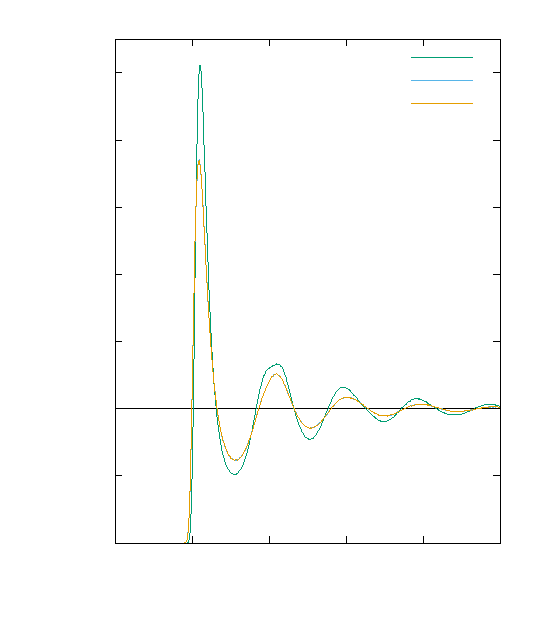
\includegraphics{rdf}}%
    \gplfronttext
  \end{picture}%
\endgroup

		\caption{}
		\label{fig:rdf864}
	\end{subfigure}%
	\begin{subfigure}[b]{0.5\textwidth}
		% GNUPLOT: LaTeX picture with Postscript
\begingroup
  \makeatletter
  \providecommand\color[2][]{%
    \GenericError{(gnuplot) \space\space\space\@spaces}{%
      Package color not loaded in conjunction with
      terminal option `colourtext'%
    }{See the gnuplot documentation for explanation.%
    }{Either use 'blacktext' in gnuplot or load the package
      color.sty in LaTeX.}%
    \renewcommand\color[2][]{}%
  }%
  \providecommand\includegraphics[2][]{%
    \GenericError{(gnuplot) \space\space\space\@spaces}{%
      Package graphicx or graphics not loaded%
    }{See the gnuplot documentation for explanation.%
    }{The gnuplot epslatex terminal needs graphicx.sty or graphics.sty.}%
    \renewcommand\includegraphics[2][]{}%
  }%
  \providecommand\rotatebox[2]{#2}%
  \@ifundefined{ifGPcolor}{%
    \newif\ifGPcolor
    \GPcolortrue
  }{}%
  \@ifundefined{ifGPblacktext}{%
    \newif\ifGPblacktext
    \GPblacktexttrue
  }{}%
  % define a \g@addto@macro without @ in the name:
  \let\gplgaddtomacro\g@addto@macro
  % define empty templates for all commands taking text:
  \gdef\gplbacktext{}%
  \gdef\gplfronttext{}%
  \makeatother
  \ifGPblacktext
    % no textcolor at all
    \def\colorrgb#1{}%
    \def\colorgray#1{}%
  \else
    % gray or color?
    \ifGPcolor
      \def\colorrgb#1{\color[rgb]{#1}}%
      \def\colorgray#1{\color[gray]{#1}}%
      \expandafter\def\csname LTw\endcsname{\color{white}}%
      \expandafter\def\csname LTb\endcsname{\color{black}}%
      \expandafter\def\csname LTa\endcsname{\color{black}}%
      \expandafter\def\csname LT0\endcsname{\color[rgb]{1,0,0}}%
      \expandafter\def\csname LT1\endcsname{\color[rgb]{0,1,0}}%
      \expandafter\def\csname LT2\endcsname{\color[rgb]{0,0,1}}%
      \expandafter\def\csname LT3\endcsname{\color[rgb]{1,0,1}}%
      \expandafter\def\csname LT4\endcsname{\color[rgb]{0,1,1}}%
      \expandafter\def\csname LT5\endcsname{\color[rgb]{1,1,0}}%
      \expandafter\def\csname LT6\endcsname{\color[rgb]{0,0,0}}%
      \expandafter\def\csname LT7\endcsname{\color[rgb]{1,0.3,0}}%
      \expandafter\def\csname LT8\endcsname{\color[rgb]{0.5,0.5,0.5}}%
    \else
      % gray
      \def\colorrgb#1{\color{black}}%
      \def\colorgray#1{\color[gray]{#1}}%
      \expandafter\def\csname LTw\endcsname{\color{white}}%
      \expandafter\def\csname LTb\endcsname{\color{black}}%
      \expandafter\def\csname LTa\endcsname{\color{black}}%
      \expandafter\def\csname LT0\endcsname{\color{black}}%
      \expandafter\def\csname LT1\endcsname{\color{black}}%
      \expandafter\def\csname LT2\endcsname{\color{black}}%
      \expandafter\def\csname LT3\endcsname{\color{black}}%
      \expandafter\def\csname LT4\endcsname{\color{black}}%
      \expandafter\def\csname LT5\endcsname{\color{black}}%
      \expandafter\def\csname LT6\endcsname{\color{black}}%
      \expandafter\def\csname LT7\endcsname{\color{black}}%
      \expandafter\def\csname LT8\endcsname{\color{black}}%
    \fi
  \fi
    \setlength{\unitlength}{0.0500bp}%
    \ifx\gptboxheight\undefined%
      \newlength{\gptboxheight}%
      \newlength{\gptboxwidth}%
      \newsavebox{\gptboxtext}%
    \fi%
    \setlength{\fboxrule}{0.5pt}%
    \setlength{\fboxsep}{1pt}%
\begin{picture}(5040.00,5760.00)%
    \gplgaddtomacro\gplbacktext{%
      \csname LTb\endcsname%%
      \put(814,704){\makebox(0,0)[r]{\strut{}$0$}}%
      \put(814,1294){\makebox(0,0)[r]{\strut{}$0.5$}}%
      \put(814,1883){\makebox(0,0)[r]{\strut{}$1$}}%
      \put(814,2473){\makebox(0,0)[r]{\strut{}$1.5$}}%
      \put(814,3063){\makebox(0,0)[r]{\strut{}$2$}}%
      \put(814,3652){\makebox(0,0)[r]{\strut{}$2.5$}}%
      \put(814,4242){\makebox(0,0)[r]{\strut{}$3$}}%
      \put(814,4831){\makebox(0,0)[r]{\strut{}$3.5$}}%
      \put(814,5421){\makebox(0,0)[r]{\strut{}$4$}}%
      \put(946,484){\makebox(0,0){\strut{}$0.5$}}%
      \put(1357,484){\makebox(0,0){\strut{}$1$}}%
      \put(1768,484){\makebox(0,0){\strut{}$1.5$}}%
      \put(2178,484){\makebox(0,0){\strut{}$2$}}%
      \put(2589,484){\makebox(0,0){\strut{}$2.5$}}%
      \put(3000,484){\makebox(0,0){\strut{}$3$}}%
      \put(3411,484){\makebox(0,0){\strut{}$3.5$}}%
      \put(3821,484){\makebox(0,0){\strut{}$4$}}%
      \put(4232,484){\makebox(0,0){\strut{}$4.5$}}%
      \put(4643,484){\makebox(0,0){\strut{}$5$}}%
    }%
    \gplgaddtomacro\gplfronttext{%
      \csname LTb\endcsname%%
      \put(209,3121){\rotatebox{-270}{\makebox(0,0){\strut{}2-point correlation}}}%
      \put(2794,154){\makebox(0,0){\strut{}radius (nm)}}%
      \csname LTb\endcsname%%
      \put(3656,5366){\makebox(0,0)[r]{\strut{}NVE}}%
      \csname LTb\endcsname%%
      \put(3656,5146){\makebox(0,0)[r]{\strut{}NVT}}%
      \csname LTb\endcsname%%
      \put(3656,4926){\makebox(0,0)[r]{\strut{}NpT}}%
    }%
    \gplbacktext
    \put(0,0){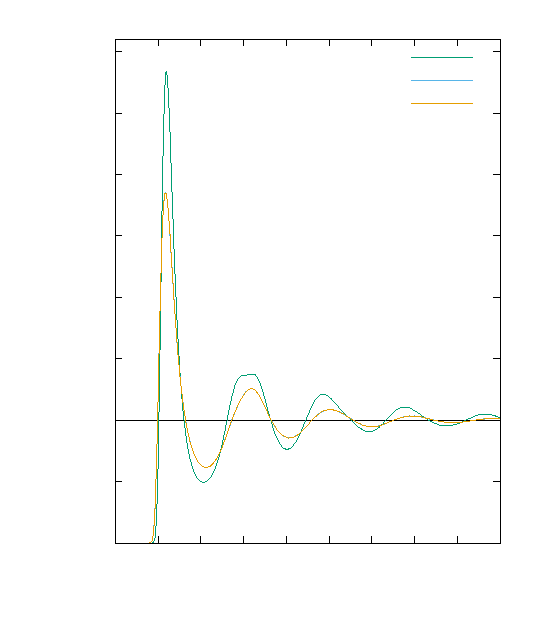
\includegraphics{rdf-1728}}%
    \gplfronttext
  \end{picture}%
\endgroup

		\caption{}
		\label{fig:rdf1728}
	\end{subfigure}
	\caption{The radial distribution function computed after a 2 ns simulation in three different ensembles, which are indicated in the legend. The radial distribution function indicates the static arrangement of the Argon atoms. The $x$-value of the peaks are indicated in Table~\ref{tab:rdfmax}. This is consistent with data obtained by Rahman~\cite{Rahman1964}.}
	\label{fig:rdf}
\end{figure}



\clearpage


\begin{table}
	\caption{The slope of the fit to the square mean displacement ($\text{nm}^2 \text{ ps}^{-1}$), which represents the diffusion coefficient.}
	\centering
	\begin{tabular}{|l|l|l|l|}
		\hline
		& NVE & NVT & NpT  \\ \hline
		864 & $4.4840\times 10^{-3}$ & $1.4058\times 10^{-2}$ & $1.4240\times 10^{-2}$  \\ \hline
		1728 & $2.9500\times 10^{-3}$ & $1.4424\times 10^{-2}$ & $1.4633\times 10^{-2}$  \\ \hline
	\end{tabular}
	\label{tab:msd}
\end{table}

\begin{figure}
	\centering
	Mean-square displacement of liquid Argon over a 2 ns for different ensembles\\
	\begin{subfigure}[b]{0.5\textwidth}
		% GNUPLOT: LaTeX picture with Postscript
\begingroup
  \makeatletter
  \providecommand\color[2][]{%
    \GenericError{(gnuplot) \space\space\space\@spaces}{%
      Package color not loaded in conjunction with
      terminal option `colourtext'%
    }{See the gnuplot documentation for explanation.%
    }{Either use 'blacktext' in gnuplot or load the package
      color.sty in LaTeX.}%
    \renewcommand\color[2][]{}%
  }%
  \providecommand\includegraphics[2][]{%
    \GenericError{(gnuplot) \space\space\space\@spaces}{%
      Package graphicx or graphics not loaded%
    }{See the gnuplot documentation for explanation.%
    }{The gnuplot epslatex terminal needs graphicx.sty or graphics.sty.}%
    \renewcommand\includegraphics[2][]{}%
  }%
  \providecommand\rotatebox[2]{#2}%
  \@ifundefined{ifGPcolor}{%
    \newif\ifGPcolor
    \GPcolortrue
  }{}%
  \@ifundefined{ifGPblacktext}{%
    \newif\ifGPblacktext
    \GPblacktexttrue
  }{}%
  % define a \g@addto@macro without @ in the name:
  \let\gplgaddtomacro\g@addto@macro
  % define empty templates for all commands taking text:
  \gdef\gplbacktext{}%
  \gdef\gplfronttext{}%
  \makeatother
  \ifGPblacktext
    % no textcolor at all
    \def\colorrgb#1{}%
    \def\colorgray#1{}%
  \else
    % gray or color?
    \ifGPcolor
      \def\colorrgb#1{\color[rgb]{#1}}%
      \def\colorgray#1{\color[gray]{#1}}%
      \expandafter\def\csname LTw\endcsname{\color{white}}%
      \expandafter\def\csname LTb\endcsname{\color{black}}%
      \expandafter\def\csname LTa\endcsname{\color{black}}%
      \expandafter\def\csname LT0\endcsname{\color[rgb]{1,0,0}}%
      \expandafter\def\csname LT1\endcsname{\color[rgb]{0,1,0}}%
      \expandafter\def\csname LT2\endcsname{\color[rgb]{0,0,1}}%
      \expandafter\def\csname LT3\endcsname{\color[rgb]{1,0,1}}%
      \expandafter\def\csname LT4\endcsname{\color[rgb]{0,1,1}}%
      \expandafter\def\csname LT5\endcsname{\color[rgb]{1,1,0}}%
      \expandafter\def\csname LT6\endcsname{\color[rgb]{0,0,0}}%
      \expandafter\def\csname LT7\endcsname{\color[rgb]{1,0.3,0}}%
      \expandafter\def\csname LT8\endcsname{\color[rgb]{0.5,0.5,0.5}}%
    \else
      % gray
      \def\colorrgb#1{\color{black}}%
      \def\colorgray#1{\color[gray]{#1}}%
      \expandafter\def\csname LTw\endcsname{\color{white}}%
      \expandafter\def\csname LTb\endcsname{\color{black}}%
      \expandafter\def\csname LTa\endcsname{\color{black}}%
      \expandafter\def\csname LT0\endcsname{\color{black}}%
      \expandafter\def\csname LT1\endcsname{\color{black}}%
      \expandafter\def\csname LT2\endcsname{\color{black}}%
      \expandafter\def\csname LT3\endcsname{\color{black}}%
      \expandafter\def\csname LT4\endcsname{\color{black}}%
      \expandafter\def\csname LT5\endcsname{\color{black}}%
      \expandafter\def\csname LT6\endcsname{\color{black}}%
      \expandafter\def\csname LT7\endcsname{\color{black}}%
      \expandafter\def\csname LT8\endcsname{\color{black}}%
    \fi
  \fi
    \setlength{\unitlength}{0.0500bp}%
    \ifx\gptboxheight\undefined%
      \newlength{\gptboxheight}%
      \newlength{\gptboxwidth}%
      \newsavebox{\gptboxtext}%
    \fi%
    \setlength{\fboxrule}{0.5pt}%
    \setlength{\fboxsep}{1pt}%
\begin{picture}(5040.00,5760.00)%
    \gplgaddtomacro\gplbacktext{%
      \csname LTb\endcsname%%
      \put(682,704){\makebox(0,0)[r]{\strut{}$0$}}%
      \put(682,1510){\makebox(0,0)[r]{\strut{}$5$}}%
      \put(682,2316){\makebox(0,0)[r]{\strut{}$10$}}%
      \put(682,3122){\makebox(0,0)[r]{\strut{}$15$}}%
      \put(682,3927){\makebox(0,0)[r]{\strut{}$20$}}%
      \put(682,4733){\makebox(0,0)[r]{\strut{}$25$}}%
      \put(682,5539){\makebox(0,0)[r]{\strut{}$30$}}%
      \put(814,484){\makebox(0,0){\strut{}$0$}}%
      \put(1771,484){\makebox(0,0){\strut{}$500$}}%
      \put(2729,484){\makebox(0,0){\strut{}$1000$}}%
      \put(3686,484){\makebox(0,0){\strut{}$1500$}}%
      \put(4643,484){\makebox(0,0){\strut{}$2000$}}%
    }%
    \gplgaddtomacro\gplfronttext{%
      \csname LTb\endcsname%%
      \put(209,3121){\rotatebox{-270}{\makebox(0,0){\strut{}Mean Square Displacement ($\text{nm}^2$)}}}%
      \put(2728,154){\makebox(0,0){\strut{}Time (ps)}}%
      \csname LTb\endcsname%%
      \put(1342,5366){\makebox(0,0)[r]{\strut{}NVE}}%
      \csname LTb\endcsname%%
      \put(1342,5146){\makebox(0,0)[r]{\strut{}NVT}}%
      \csname LTb\endcsname%%
      \put(1342,4926){\makebox(0,0)[r]{\strut{}NpT}}%
    }%
    \gplbacktext
    \put(0,0){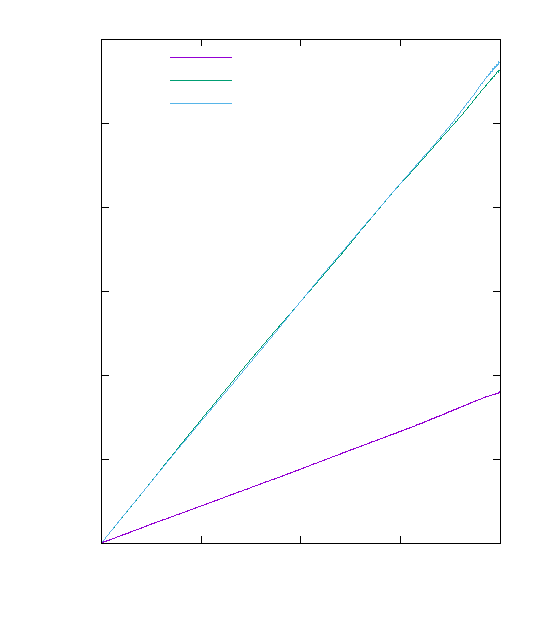
\includegraphics{msd}}%
    \gplfronttext
  \end{picture}%
\endgroup

		\caption{}
		\label{fig:msd864}
	\end{subfigure}%
	\begin{subfigure}[b]{0.5\textwidth}
		% GNUPLOT: LaTeX picture with Postscript
\begingroup
  \makeatletter
  \providecommand\color[2][]{%
    \GenericError{(gnuplot) \space\space\space\@spaces}{%
      Package color not loaded in conjunction with
      terminal option `colourtext'%
    }{See the gnuplot documentation for explanation.%
    }{Either use 'blacktext' in gnuplot or load the package
      color.sty in LaTeX.}%
    \renewcommand\color[2][]{}%
  }%
  \providecommand\includegraphics[2][]{%
    \GenericError{(gnuplot) \space\space\space\@spaces}{%
      Package graphicx or graphics not loaded%
    }{See the gnuplot documentation for explanation.%
    }{The gnuplot epslatex terminal needs graphicx.sty or graphics.sty.}%
    \renewcommand\includegraphics[2][]{}%
  }%
  \providecommand\rotatebox[2]{#2}%
  \@ifundefined{ifGPcolor}{%
    \newif\ifGPcolor
    \GPcolortrue
  }{}%
  \@ifundefined{ifGPblacktext}{%
    \newif\ifGPblacktext
    \GPblacktexttrue
  }{}%
  % define a \g@addto@macro without @ in the name:
  \let\gplgaddtomacro\g@addto@macro
  % define empty templates for all commands taking text:
  \gdef\gplbacktext{}%
  \gdef\gplfronttext{}%
  \makeatother
  \ifGPblacktext
    % no textcolor at all
    \def\colorrgb#1{}%
    \def\colorgray#1{}%
  \else
    % gray or color?
    \ifGPcolor
      \def\colorrgb#1{\color[rgb]{#1}}%
      \def\colorgray#1{\color[gray]{#1}}%
      \expandafter\def\csname LTw\endcsname{\color{white}}%
      \expandafter\def\csname LTb\endcsname{\color{black}}%
      \expandafter\def\csname LTa\endcsname{\color{black}}%
      \expandafter\def\csname LT0\endcsname{\color[rgb]{1,0,0}}%
      \expandafter\def\csname LT1\endcsname{\color[rgb]{0,1,0}}%
      \expandafter\def\csname LT2\endcsname{\color[rgb]{0,0,1}}%
      \expandafter\def\csname LT3\endcsname{\color[rgb]{1,0,1}}%
      \expandafter\def\csname LT4\endcsname{\color[rgb]{0,1,1}}%
      \expandafter\def\csname LT5\endcsname{\color[rgb]{1,1,0}}%
      \expandafter\def\csname LT6\endcsname{\color[rgb]{0,0,0}}%
      \expandafter\def\csname LT7\endcsname{\color[rgb]{1,0.3,0}}%
      \expandafter\def\csname LT8\endcsname{\color[rgb]{0.5,0.5,0.5}}%
    \else
      % gray
      \def\colorrgb#1{\color{black}}%
      \def\colorgray#1{\color[gray]{#1}}%
      \expandafter\def\csname LTw\endcsname{\color{white}}%
      \expandafter\def\csname LTb\endcsname{\color{black}}%
      \expandafter\def\csname LTa\endcsname{\color{black}}%
      \expandafter\def\csname LT0\endcsname{\color{black}}%
      \expandafter\def\csname LT1\endcsname{\color{black}}%
      \expandafter\def\csname LT2\endcsname{\color{black}}%
      \expandafter\def\csname LT3\endcsname{\color{black}}%
      \expandafter\def\csname LT4\endcsname{\color{black}}%
      \expandafter\def\csname LT5\endcsname{\color{black}}%
      \expandafter\def\csname LT6\endcsname{\color{black}}%
      \expandafter\def\csname LT7\endcsname{\color{black}}%
      \expandafter\def\csname LT8\endcsname{\color{black}}%
    \fi
  \fi
    \setlength{\unitlength}{0.0500bp}%
    \ifx\gptboxheight\undefined%
      \newlength{\gptboxheight}%
      \newlength{\gptboxwidth}%
      \newsavebox{\gptboxtext}%
    \fi%
    \setlength{\fboxrule}{0.5pt}%
    \setlength{\fboxsep}{1pt}%
\begin{picture}(5040.00,5760.00)%
    \gplgaddtomacro\gplbacktext{%
      \csname LTb\endcsname%%
      \put(682,704){\makebox(0,0)[r]{\strut{}$0$}}%
      \put(682,1510){\makebox(0,0)[r]{\strut{}$5$}}%
      \put(682,2316){\makebox(0,0)[r]{\strut{}$10$}}%
      \put(682,3122){\makebox(0,0)[r]{\strut{}$15$}}%
      \put(682,3927){\makebox(0,0)[r]{\strut{}$20$}}%
      \put(682,4733){\makebox(0,0)[r]{\strut{}$25$}}%
      \put(682,5539){\makebox(0,0)[r]{\strut{}$30$}}%
      \put(814,484){\makebox(0,0){\strut{}$0$}}%
      \put(1771,484){\makebox(0,0){\strut{}$500$}}%
      \put(2729,484){\makebox(0,0){\strut{}$1000$}}%
      \put(3686,484){\makebox(0,0){\strut{}$1500$}}%
      \put(4643,484){\makebox(0,0){\strut{}$2000$}}%
    }%
    \gplgaddtomacro\gplfronttext{%
      \csname LTb\endcsname%%
      \put(209,3121){\rotatebox{-270}{\makebox(0,0){\strut{}Mean Square Displacement ($\text{nm}^2$)}}}%
      \put(2728,154){\makebox(0,0){\strut{}Time (ps)}}%
      \csname LTb\endcsname%%
      \put(1342,5366){\makebox(0,0)[r]{\strut{}NVE}}%
      \csname LTb\endcsname%%
      \put(1342,5146){\makebox(0,0)[r]{\strut{}NVT}}%
      \csname LTb\endcsname%%
      \put(1342,4926){\makebox(0,0)[r]{\strut{}NpT}}%
    }%
    \gplbacktext
    \put(0,0){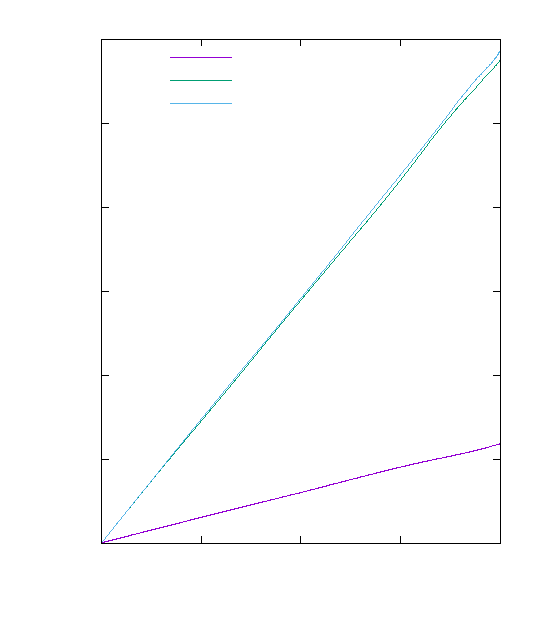
\includegraphics{msd-1728}}%
    \gplfronttext
  \end{picture}%
\endgroup

		\caption{}
		\label{fig:msd1728}
	\end{subfigure}
	\caption{The mean square displacement over the entire simulation is displayed. As expected, it follows a linear trajectory. The diffusion coefficients corresponding to each ensemble and for the two different particle numbers are displayed in Table~\ref{tab:msd}. In the case of the NVE ensemble, the slope corresponds to a diffusion coefficient of }
	\label{fig:msd}
\end{figure}




\begin{figure}
	\centering
	Velocity auto-correlation of liquid Argon over a 2 ns for different ensembles\\
	\begin{subfigure}[b]{0.5\textwidth}
		% GNUPLOT: LaTeX picture with Postscript
\begingroup
  \makeatletter
  \providecommand\color[2][]{%
    \GenericError{(gnuplot) \space\space\space\@spaces}{%
      Package color not loaded in conjunction with
      terminal option `colourtext'%
    }{See the gnuplot documentation for explanation.%
    }{Either use 'blacktext' in gnuplot or load the package
      color.sty in LaTeX.}%
    \renewcommand\color[2][]{}%
  }%
  \providecommand\includegraphics[2][]{%
    \GenericError{(gnuplot) \space\space\space\@spaces}{%
      Package graphicx or graphics not loaded%
    }{See the gnuplot documentation for explanation.%
    }{The gnuplot epslatex terminal needs graphicx.sty or graphics.sty.}%
    \renewcommand\includegraphics[2][]{}%
  }%
  \providecommand\rotatebox[2]{#2}%
  \@ifundefined{ifGPcolor}{%
    \newif\ifGPcolor
    \GPcolortrue
  }{}%
  \@ifundefined{ifGPblacktext}{%
    \newif\ifGPblacktext
    \GPblacktexttrue
  }{}%
  % define a \g@addto@macro without @ in the name:
  \let\gplgaddtomacro\g@addto@macro
  % define empty templates for all commands taking text:
  \gdef\gplbacktext{}%
  \gdef\gplfronttext{}%
  \makeatother
  \ifGPblacktext
    % no textcolor at all
    \def\colorrgb#1{}%
    \def\colorgray#1{}%
  \else
    % gray or color?
    \ifGPcolor
      \def\colorrgb#1{\color[rgb]{#1}}%
      \def\colorgray#1{\color[gray]{#1}}%
      \expandafter\def\csname LTw\endcsname{\color{white}}%
      \expandafter\def\csname LTb\endcsname{\color{black}}%
      \expandafter\def\csname LTa\endcsname{\color{black}}%
      \expandafter\def\csname LT0\endcsname{\color[rgb]{1,0,0}}%
      \expandafter\def\csname LT1\endcsname{\color[rgb]{0,1,0}}%
      \expandafter\def\csname LT2\endcsname{\color[rgb]{0,0,1}}%
      \expandafter\def\csname LT3\endcsname{\color[rgb]{1,0,1}}%
      \expandafter\def\csname LT4\endcsname{\color[rgb]{0,1,1}}%
      \expandafter\def\csname LT5\endcsname{\color[rgb]{1,1,0}}%
      \expandafter\def\csname LT6\endcsname{\color[rgb]{0,0,0}}%
      \expandafter\def\csname LT7\endcsname{\color[rgb]{1,0.3,0}}%
      \expandafter\def\csname LT8\endcsname{\color[rgb]{0.5,0.5,0.5}}%
    \else
      % gray
      \def\colorrgb#1{\color{black}}%
      \def\colorgray#1{\color[gray]{#1}}%
      \expandafter\def\csname LTw\endcsname{\color{white}}%
      \expandafter\def\csname LTb\endcsname{\color{black}}%
      \expandafter\def\csname LTa\endcsname{\color{black}}%
      \expandafter\def\csname LT0\endcsname{\color{black}}%
      \expandafter\def\csname LT1\endcsname{\color{black}}%
      \expandafter\def\csname LT2\endcsname{\color{black}}%
      \expandafter\def\csname LT3\endcsname{\color{black}}%
      \expandafter\def\csname LT4\endcsname{\color{black}}%
      \expandafter\def\csname LT5\endcsname{\color{black}}%
      \expandafter\def\csname LT6\endcsname{\color{black}}%
      \expandafter\def\csname LT7\endcsname{\color{black}}%
      \expandafter\def\csname LT8\endcsname{\color{black}}%
    \fi
  \fi
    \setlength{\unitlength}{0.0500bp}%
    \ifx\gptboxheight\undefined%
      \newlength{\gptboxheight}%
      \newlength{\gptboxwidth}%
      \newsavebox{\gptboxtext}%
    \fi%
    \setlength{\fboxrule}{0.5pt}%
    \setlength{\fboxsep}{1pt}%
\begin{picture}(5040.00,5760.00)%
    \gplgaddtomacro\gplbacktext{%
      \csname LTb\endcsname%%
      \put(946,704){\makebox(0,0)[r]{\strut{}$-0.2$}}%
      \put(946,1510){\makebox(0,0)[r]{\strut{}$0$}}%
      \put(946,2316){\makebox(0,0)[r]{\strut{}$0.2$}}%
      \put(946,3122){\makebox(0,0)[r]{\strut{}$0.4$}}%
      \put(946,3927){\makebox(0,0)[r]{\strut{}$0.6$}}%
      \put(946,4733){\makebox(0,0)[r]{\strut{}$0.8$}}%
      \put(946,5539){\makebox(0,0)[r]{\strut{}$1$}}%
      \put(1078,484){\makebox(0,0){\strut{}$0$}}%
      \put(1791,484){\makebox(0,0){\strut{}$2$}}%
      \put(2504,484){\makebox(0,0){\strut{}$4$}}%
      \put(3217,484){\makebox(0,0){\strut{}$6$}}%
      \put(3930,484){\makebox(0,0){\strut{}$8$}}%
      \put(4643,484){\makebox(0,0){\strut{}$10$}}%
    }%
    \gplgaddtomacro\gplfronttext{%
      \csname LTb\endcsname%%
      \put(209,3121){\rotatebox{-270}{\makebox(0,0){\strut{}Velocity Auto-Correlation ($\text{nm}^2$)}}}%
      \put(2860,154){\makebox(0,0){\strut{}Time (ps)}}%
      \csname LTb\endcsname%%
      \put(3656,5366){\makebox(0,0)[r]{\strut{}NVE}}%
      \csname LTb\endcsname%%
      \put(3656,5146){\makebox(0,0)[r]{\strut{}NVT}}%
      \csname LTb\endcsname%%
      \put(3656,4926){\makebox(0,0)[r]{\strut{}NpT}}%
    }%
    \gplbacktext
    \put(0,0){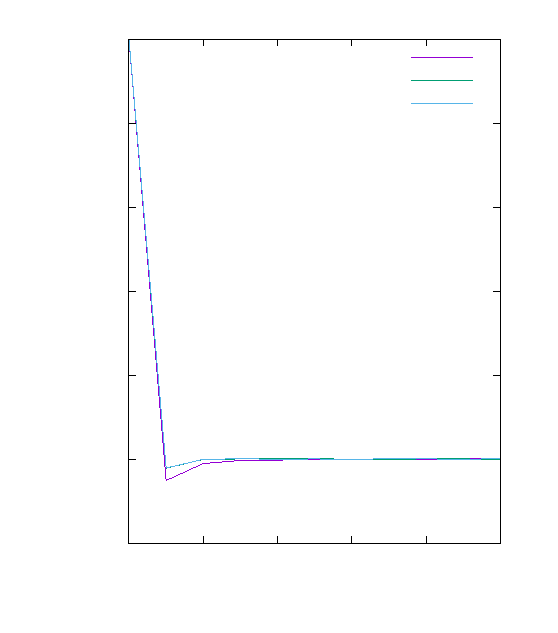
\includegraphics{velacc}}%
    \gplfronttext
  \end{picture}%
\endgroup

		\caption{}
		\label{fig:velacc864}
	\end{subfigure}%
	\begin{subfigure}[b]{0.5\textwidth}
		% GNUPLOT: LaTeX picture with Postscript
\begingroup
  \makeatletter
  \providecommand\color[2][]{%
    \GenericError{(gnuplot) \space\space\space\@spaces}{%
      Package color not loaded in conjunction with
      terminal option `colourtext'%
    }{See the gnuplot documentation for explanation.%
    }{Either use 'blacktext' in gnuplot or load the package
      color.sty in LaTeX.}%
    \renewcommand\color[2][]{}%
  }%
  \providecommand\includegraphics[2][]{%
    \GenericError{(gnuplot) \space\space\space\@spaces}{%
      Package graphicx or graphics not loaded%
    }{See the gnuplot documentation for explanation.%
    }{The gnuplot epslatex terminal needs graphicx.sty or graphics.sty.}%
    \renewcommand\includegraphics[2][]{}%
  }%
  \providecommand\rotatebox[2]{#2}%
  \@ifundefined{ifGPcolor}{%
    \newif\ifGPcolor
    \GPcolortrue
  }{}%
  \@ifundefined{ifGPblacktext}{%
    \newif\ifGPblacktext
    \GPblacktexttrue
  }{}%
  % define a \g@addto@macro without @ in the name:
  \let\gplgaddtomacro\g@addto@macro
  % define empty templates for all commands taking text:
  \gdef\gplbacktext{}%
  \gdef\gplfronttext{}%
  \makeatother
  \ifGPblacktext
    % no textcolor at all
    \def\colorrgb#1{}%
    \def\colorgray#1{}%
  \else
    % gray or color?
    \ifGPcolor
      \def\colorrgb#1{\color[rgb]{#1}}%
      \def\colorgray#1{\color[gray]{#1}}%
      \expandafter\def\csname LTw\endcsname{\color{white}}%
      \expandafter\def\csname LTb\endcsname{\color{black}}%
      \expandafter\def\csname LTa\endcsname{\color{black}}%
      \expandafter\def\csname LT0\endcsname{\color[rgb]{1,0,0}}%
      \expandafter\def\csname LT1\endcsname{\color[rgb]{0,1,0}}%
      \expandafter\def\csname LT2\endcsname{\color[rgb]{0,0,1}}%
      \expandafter\def\csname LT3\endcsname{\color[rgb]{1,0,1}}%
      \expandafter\def\csname LT4\endcsname{\color[rgb]{0,1,1}}%
      \expandafter\def\csname LT5\endcsname{\color[rgb]{1,1,0}}%
      \expandafter\def\csname LT6\endcsname{\color[rgb]{0,0,0}}%
      \expandafter\def\csname LT7\endcsname{\color[rgb]{1,0.3,0}}%
      \expandafter\def\csname LT8\endcsname{\color[rgb]{0.5,0.5,0.5}}%
    \else
      % gray
      \def\colorrgb#1{\color{black}}%
      \def\colorgray#1{\color[gray]{#1}}%
      \expandafter\def\csname LTw\endcsname{\color{white}}%
      \expandafter\def\csname LTb\endcsname{\color{black}}%
      \expandafter\def\csname LTa\endcsname{\color{black}}%
      \expandafter\def\csname LT0\endcsname{\color{black}}%
      \expandafter\def\csname LT1\endcsname{\color{black}}%
      \expandafter\def\csname LT2\endcsname{\color{black}}%
      \expandafter\def\csname LT3\endcsname{\color{black}}%
      \expandafter\def\csname LT4\endcsname{\color{black}}%
      \expandafter\def\csname LT5\endcsname{\color{black}}%
      \expandafter\def\csname LT6\endcsname{\color{black}}%
      \expandafter\def\csname LT7\endcsname{\color{black}}%
      \expandafter\def\csname LT8\endcsname{\color{black}}%
    \fi
  \fi
    \setlength{\unitlength}{0.0500bp}%
    \ifx\gptboxheight\undefined%
      \newlength{\gptboxheight}%
      \newlength{\gptboxwidth}%
      \newsavebox{\gptboxtext}%
    \fi%
    \setlength{\fboxrule}{0.5pt}%
    \setlength{\fboxsep}{1pt}%
\begin{picture}(5040.00,5760.00)%
    \gplgaddtomacro\gplbacktext{%
      \csname LTb\endcsname%%
      \put(946,704){\makebox(0,0)[r]{\strut{}$-0.2$}}%
      \put(946,1510){\makebox(0,0)[r]{\strut{}$0$}}%
      \put(946,2316){\makebox(0,0)[r]{\strut{}$0.2$}}%
      \put(946,3122){\makebox(0,0)[r]{\strut{}$0.4$}}%
      \put(946,3927){\makebox(0,0)[r]{\strut{}$0.6$}}%
      \put(946,4733){\makebox(0,0)[r]{\strut{}$0.8$}}%
      \put(946,5539){\makebox(0,0)[r]{\strut{}$1$}}%
      \put(1078,484){\makebox(0,0){\strut{}$0$}}%
      \put(1791,484){\makebox(0,0){\strut{}$2$}}%
      \put(2504,484){\makebox(0,0){\strut{}$4$}}%
      \put(3217,484){\makebox(0,0){\strut{}$6$}}%
      \put(3930,484){\makebox(0,0){\strut{}$8$}}%
      \put(4643,484){\makebox(0,0){\strut{}$10$}}%
    }%
    \gplgaddtomacro\gplfronttext{%
      \csname LTb\endcsname%%
      \put(209,3121){\rotatebox{-270}{\makebox(0,0){\strut{}Velocity Auto-Correlation ($\text{nm}^2$)}}}%
      \put(2860,154){\makebox(0,0){\strut{}Time (ps)}}%
      \csname LTb\endcsname%%
      \put(3656,5366){\makebox(0,0)[r]{\strut{}NVE}}%
      \csname LTb\endcsname%%
      \put(3656,5146){\makebox(0,0)[r]{\strut{}NVT}}%
      \csname LTb\endcsname%%
      \put(3656,4926){\makebox(0,0)[r]{\strut{}NpT}}%
    }%
    \gplbacktext
    \put(0,0){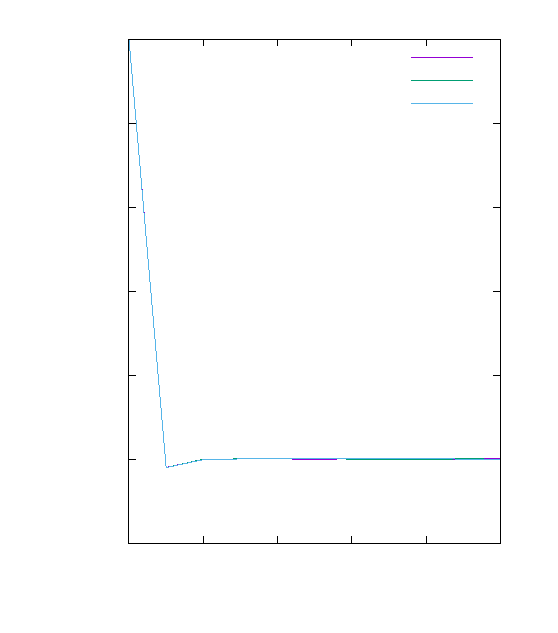
\includegraphics{velacc-1728}}%
    \gplfronttext
  \end{picture}%
\endgroup

		\caption{}
		\label{fig:velacc1728}
	\end{subfigure}
	\caption{The velocity auto-correlation function is displayed, up to the first 10 ps. Even from the first 3 ps, the velocity auto-correlation function takes values close to zero (meaning there's no correlation in subsequent time indices). }
	\label{fig:velacc}
\end{figure}

\clearpage

\section{Discussion}

In general, very good correspondence was achieved with the results from Rahman~\cite{Rahman1964}. Those results are also consistent with argon experiments from the time. For instance, the radial distribution function data where the peaks are found (that is, the values of $|\vec{r}|/\sigma$) are consistent with the data from Rahman. The velocity auto-correlation function, though plotted with fewer values, exhibits the same qualitative shape as determined by Rahman. The exception is the diffusion constant determined from the mean-squared displacement, which are different from Rahman; the values in this work are also inconsistent with the experiment from Naghizadeh and Rice~\cite{Naghizadeh1962}.

In the future, the Argon simulation should be rerun and different types of data collected, such as the dynamic structure factor, and at different temperatures, in order to match to existing experiment. One example is the work by Sk\"old and co-workers which measured the scattering functions for liquid Argon at 85.2 K~\cite{Skoeld1972}, and similar work by Yarnell~\cite{Yarnell1973}.
Furthermore, the particle type can even be interchanged to compare to other experiments, such as the work by Svensson and co-workers on liquid Helium which measured the dynamic structure factor~\cite{Svensson1980}.

\clearpage


%% If you have bibdatabase file and want bibtex to generate the
%% bibitems, please use
%%
\bibliographystyle{elsarticle-num} 
\bibliography{C:\\Users\\Zirconix\\Dropbox\\research\\@refs\\assignments.bib,C:\\Users\\Zirconix\\Dropbox\\research\\@refs\\jabrefs.bib}
%%  \bibliography{<your bibdatabase>}

%% else use the following coding to input the bibitems directly in the
%% TeX file.

\end{document}
\endinput
%%
%% End of file `elsarticle-template-num.tex'.

